\section{Vehicle}\label{Vehicle}
\texttt{Vehicle} klassen representerer et køretøj i programmet, og indeholder den offentlige metode \texttt{Drive}, som \texttt{Simulation} klassen bruger til at køre alle bilerne. 

\begin{figure}[H]
\begin{lstlisting}
public Vehicle(Project project, Node home, Destination dest, 
               VehicleType type, int toDestTime, int toHomeTime)
\end{lstlisting}
\caption{Vehicle Constructor parametre}\label{VehicleConstructor}
\end{figure}

Constructoren til \texttt{Vehicle} tager imod en række forskellige parametre som ses på figur \ref{VehicleConstructor}, og udfører nogle opgaver, så køretøjet er klar til at køre. Som figur \ref{VehicleConstructor} viser, så tager klassen imod et \texttt{Project}, dette bliver ikke gemt i selve \texttt{Vehicle} klassen, men det bruges til at finde den nærmeste parkings plads, eller en tilfældig \texttt{Node} med typen \texttt{Outbound}. Efter at have fundet slut punktet, bliver \texttt{\_toDestPath} og \texttt{\_toHomePath} fundet gennem \texttt{Pathfinder} klassen. \texttt{toDestTime} er den tid køretøjet skal begynde at køre mod destinationen, og \texttt{toHomeTime} er den tid hvor den skal begynde at køre tilbage igen. Sidst sættes \texttt{bool} variablen \texttt{Active} til at være \texttt{false}.

\begin{figure}[H]
\begin{lstlisting}
public void Drive(int time)
{
  if (!Active) CheckActive(time);
  else
  {
    Speed = GetSpeed();
    if (Speed != 0)
      Move(MathExtension.KmhToMms(Speed) * _settings.StepSize);
    if (time % Simulation.RecordInterval == 0 
        && !_toHomeStarted)
      ToDestRecord.Add(new PointD(Position));
    else if (time % Simulation.RecordInterval == 0 
             && _toHomeStarted)
      ToHomeRecord.Add(new PointD(Position));
  }
}
\end{lstlisting}
\caption{Drive metoden}\label{DriveCode}
\end{figure}

Som afsnit \ref{SimulationClass} beskriver, bliver \texttt{Drive} kaldt for hver \texttt{Vehicle} instans, hver gang simulationen tager et step. I \texttt{Drive} metoden som vist på figur \ref{DriveCode}, bliver der først tjekket om køretøjet er aktivt, hvis ikke kaldes \texttt{CheckActive}, der ser om tiden er højere end det tidspunkt hvor køretøjet skal begynde at køre, og hvis det er sandt vil køretøjet så aktiveres. I tilfældet at køretøjet allerede er aktivt, findes hastigheden bilen skal køre gennem metoden \texttt{GetSpeed}, og derefter hvis hastigheden ikke er nul, vil køretøjet flytte sig en afstand baseret på køretøjets nuværende hastighed. Efter køretøjet har bevæget sig, vil positionen blive gemt i enten \texttt{ToDestRecord} eller \texttt{ToHomeRecord}, alt efter hvilken rute der bliver kørt på tidspunktet. Positionen bliver kun gemt hver gang tiden kan gå lige op med konstaten \texttt{Simulation.RecordInterval}, det vil sige at positionen kun bliver gemt 10 gange i sekundet, selvom step størrelsen godt kunne være mindre. Grunden til at der ikke bare bliver gemt hver gang biler har flyttet sig, er at simulationen vil kræve alt for meget hukommelse.

\begin{figure}[H]
\begin{lstlisting}
private double GetSpeed()
{
  int incomingVehiclesCount = _currentRoad.To
                              .IncomingVehicles.Count;
  Vehicle vehicleInfront = VehicleInfront(_settings.VehicleSpace);
  if (CurrentNode != null 
      && CurrentNode.Type == NodeTypes.Light 
      && !CurrentNode.Green)
    return 0;
  else if (CurrentNode != null 
           && CurrentNode.Type == NodeTypes.Yield
           && incomingVehiclesCount > 0 
           && !(incomingVehiclesCount == 1 
           && _currentRoad.To.IncomingVehicles.Contains(this)))
    return 0;
  else if (vehicleInfront != null)
    return vehicleInfront.Speed;
  else
  {
    if (Type.MaxSpeed > _currentRoad.Type.Speed)
      return _currentRoad.Type.Speed;
    else
      return Type.MaxSpeed;
  }
}
\end{lstlisting}
\caption{GetSpeed metoden}\label{GetSpeedCode}
\end{figure}

På figur \ref{GetSpeedCode} vises metoden \texttt{GetSpeed}, som var den første der blev kaldet i \texttt{Drive} metoden. Først tjekkes der på linje 6, om køretøjet er på en \texttt{Node}, (\texttt{CurrentNode} er null hvis køretøjet er på en vej mellem to noder), og hvis den \texttt{Node} så har typen \texttt{Light}, og at \texttt{bool} variablen \texttt{Green} er false, svarer det til at køretøjet er ved et rødt lys, og hastigheden bliver dermed returneret som et 0. Derefter tjekkes der på linje 10, om \texttt{Noden} har typen \texttt{Yield}. Hvis det er sandt, og at der er indkommende køretøjer som ikke er dette køretøj, så vil hastigheden også sættes til 0. Hvis ikke de to første er sande, så tjekkes der efter om der er et køretøj foran dette køretøj indenfor rækkeviden \texttt{VehicleSpace}, som brugeren kan indstille i settings. Hvis der findes et køretøj, bliver hastigheden sat lig med køretøjet. Sidst har vi tilfældet hvor der ikke er noget der blokerer køretøjet, hvor hastigheden vil blive sat lig hastighedsgrænsen på vejen, medmindre køretøjets egen max hastighed er lavere hvor hastigheden bare vil sættes til det maksimale.

\begin{figure}[H]
\begin{lstlisting}
private void Move(double distanceToMove)
{
  CurrentNode = null;
  TranslateVehicle(distanceToMove);
  ControlOverreach();
  ShowAsIncoming();
}
\end{lstlisting}
\caption{Move metoden}\label{MoveCode}
\end{figure}

Figur \ref{MoveCode} viser \texttt{Move} metoden. Som navnet indikerer, bruges metoden til at flytte køretøjet. Først bliver \texttt{CurrentNode} sat til null, da Move metoden aldrig bliver kaldet med en distance på 0, og vil dermed altid flytte sig fra den nuværende \texttt{Node}. 

\begin{wrapfigure}{r}{0.5\textwidth}
    \centering
    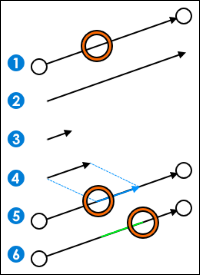
\includegraphics[width=4cm,keepaspectratio]{Pictures/Implementation/TranslateVehicle}
    \caption{TranslateVehicle}
    \label{TranslateVehicle}
\end{wrapfigure}

\vspace{5mm}

Derefter kaldes \texttt{TranslateVehicle}, hvilket er en metode der flytter køretøjet i retningen af vejen, uden at overveje om den har kørt for langt. Måden metoden gør dette på er illustreret på figur \ref{TranslateVehicle}.

\begin{enumerate}
\item Et køretøj på en vej
\item Vejen laves om til en vektor
\item Vej-Vektoren laves til en unit vektor
\item Vektoren skaleres med afstanden der skal køres
\item Vektorens X og Y koordinater bliver adderet til positionen på køretøjet
\item Køretøjet har flyttet sig
\end{enumerate}

\begin{figure}[H]
\begin{lstlisting}
private void ControlOverreach()
{
  double currentRoadStartDistance = MathExtension
    .Distance(Position, new PointD(_currentRoad.From.Position));
  if (currentRoadStartDistance > _currentRoad.Length)
  {
    if (_currentPathIndex + 1 == _currentPath.Count)
      Deactivate();
    else if (_currentRoad.To.Type == NodeTypes.Light 
             || _currentRoad.To.Type == NodeTypes.Yield)
      GoToNextRoad();
    else
    {
      double remainingDistanceToMove = currentRoadStartDistance 
                                       - _currentRoad.Length;
      GoToNextRoad();
      Move(remainingDistanceToMove);
    }
  }
}
\end{lstlisting}
\caption{ControlOverreach metoden}\label{ControlOverreachCode}
\end{figure}

Efter \texttt{TranslateVehicle} har flyttet køretøjet, bruges \texttt{ControlOverreach} til at tjekke om der er blevet kørt for langt, altså udover enden af vejen. Det findes ved at udregne distancen til knuden der ligger i starten af den nuværende vej \texttt{(CurrentRoad)}, og hvis den er længere end vejen så må køretøjet have kørt for langt. Når der er kørt for langt, tjekkes der først om køretøjet er ved slutningen af ruten, hvor den så vil deaktiverer, ellers hvis slutknuden på den nuværende vej er af typen \texttt{Light} eller \texttt{Yield}, standser køretøjet bare på punktet, hvor der så i næste step vil skulle tjekkes om den må køre videre. Sidst hvis køretøjet gerne må fortsætte, findes den afstand der er blevet kørt for langt med, køretøjet sættes ind på den næste \texttt{Road} på \texttt{CurrentPath}, og \texttt{Move} bliver kaldet igen.

\vspace{5mm}

Som det sidste der sker i \texttt{Move} metoden, har vi metoden \texttt{ShowAsIncomming}, der sætter køretøjet på en liste af indkommende biler på knuderne foran, hvis de er indenfor en afstand brugeren kan sætte i indstillingerne. Dette bruges når andre køretøj skal vurdere om de må køre ved en \texttt{Node} med typen \texttt{Yield} (vigeplight).